\subsection{Attack Models}\label{sec:cryptographic_security_overview:attack_model}

With a threat model, it is possible to accordingly derive an \textbf{attack model} for mathematical and algorithmic attacks describing specific methods or approaches attackers may employ to (usually) retrieve (portions of) private or secret keys through cryptanalysis (\Cref{sec:cryptography_basics}).

\remarkBlock{Threat models vs. attack models}{Threat models establish the capabilities and resources of attackers, while attack models operate within the constraints of a given threat model. Hence, depending on the threat model, attack models may be more or less powerful (\Cref{fig:attack_model_relationship}).}

Some common attack models are:

\begin{itemize}
	\item \textbf{\gls{coa}}: attackers have access to one or more ciphertexts only and not to the corresponding plaintexts. Brute force attacks or exhaustive key search attacks (\Cref{sec:cryptographic_security_overview:attacks}) are attacks in the \gls{coa} attack model;
	\item \textbf{\gls{kpa}}: attackers have access to a limited number of ciphertext-plaintext pairs;
	\item \textbf{\gls{cpa}}: attackers can choose a number of plaintexts for which obtain the corresponding ciphertext. The possibility to choose arbitrary plaintexts allows attackers to explore edge cases and trigger particularly significant behaviors. The \gls{cpa} attack model entails that the attacker has access to a so-called \textbf{encryption oracle}.\footnote{The term ``oracle'' indicates a black-box function available for use (in this case, by the attacker) whose inner functioning is, however, opaque. For example, an encryption oracle allows for encrypting any plaintext, while a decryption oracle allows for decrypting any ciphertext --- but not accessing private or secret keys. The term oracle comes from the idea of a mythological oracle, an all-knowing entity accepting questions and replying the truth.} The \textbf{\gls{cpa2}} derives from \gls{cpa} and extends it by allowing attackers to choose plaintexts adaptively, i.e., attackers can choose plaintexts based on previous ciphertext-plaintext pairs observed. Consequently, \gls{cpa} is also referred to as \textbf{CPA1};
	\item \textbf{\gls{cca}}: attackers can choose a number of ciphertexts of which receive the corresponding plaintext. The \gls{cca} attack model entails that the attacker has access to a so-called \textbf{decryption oracle}. The \textbf{\gls{cca2}} derives from \gls{cca} and extends it by allowing attackers to choose ciphertexts adaptively, i.e., attackers can choose ciphertexts based on previous ciphertext-plaintext pairs observed. Consequently, \gls{cca} is also referred to as \textbf{CCA1}.
	\exampleBlock{A real-world example of a \gls{cca2} attack}{A practical attack in the \gls{cca2} attack model is the Bleichenbacher attack \cite{bleichenbacher_chosen_1998} against the \gls{rsa} encryption standard \gls{pkcs}\#1 \cite{rfc8017} --- see also \url{https://royalholloway.ac.uk/media/9116/gageboyleisg.pdf}.}
	\remarkBlock{\gls{cca} and \gls{cpa}}{\gls{cca} usually includes \gls{cpa}, although some distinguish the two attack models and refer to their combination as \textbf{chosen-plaintext/ciphertext attack}.}
\end{itemize}

\begin{figure}[t!]
	\begin{center}
		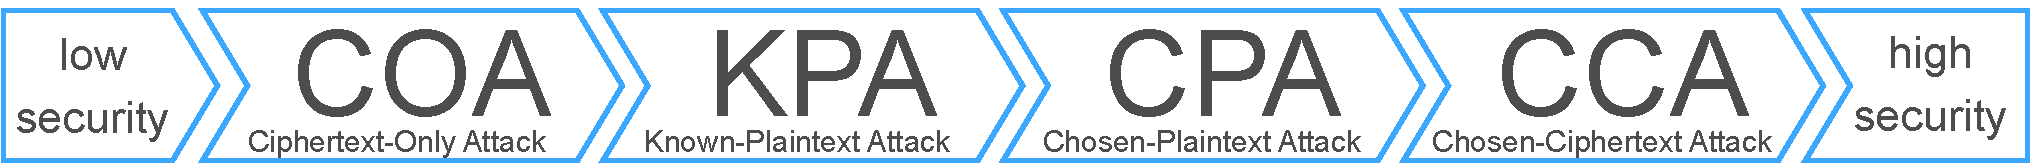
\includegraphics[width=1\linewidth]{resources/pdf/attack_model_relationship.pdf}
		\caption{The \gls{coa} attack model requires the most effort and skills by attackers to be successful; if a system resists an attacker operating in the \gls{coa} model, then it provides low security. Conversely, the \gls{cca} attack model requires the least effort and skills by attackers to be successful; if an system resists an attacker operating in the \gls{cca} model, then it provides high security.}
		\label{fig:attack_model_relationship}
	\end{center}
\end{figure}

\remarkBlock{Attack models for symmetric and asymmetric cryptography}{Attackers cannot create ciphertexts in symmetric cryptography (\Cref{sec:symmetric_cryptography}), as symmetric keys are secret. Conversely, attackers can create ciphertexts in asymmetric cryptography (\Cref{sec:asymmetric_cryptography}), as public keys are known. Hence, symmetric cryptography does not typically require security against attackers operating in the \gls{cca} attack model --- although the most secure symmetric ciphers do.}


\subsubsection{Security Goals}\label{sec:cryptographic_security_overview:attack_model:security_goals}

Attack models can be paired with (ideally any) security goals. Some common security goals are:

\begin{itemize}
	\item \textbf{\gls{ind}}: consider a ciphertext $c$ obtained by applying an algorithm to one plaintext randomly chosen among two plaintexts $m1$ and $m2$ defined by an attacker. An algorithm achieves the indistinguishability goal if the attacker --- given $c$ --- cannot determine which plaintext was chosen to produce $c$ with probability significantly better than that of random guessing (intuitively, if an attacker could determine which plaintext was used, it would mean that the ciphertext leaks information about the plaintext);
	\remarkBlock{Naming the combination of an attack model with a security goal}{The combination of an attack model with a security goal is usually denoted with the hyphenation of their acronyms (e.g., \gls{ind}-\gls{cpa} is the indistinguishability security goal under the \gls{cpa} attack model).}
	\exampleBlock{Indistinguishability and attack models}{\gls{ind}-\gls{cpa} means that the attacker can preliminarily choose a number of plaintexts for which obtain the corresponding ciphertext both before and after executing the algorithm over either $m1$ or $m2$ to obtain $c$. Similarly, \gls{ind}-\gls{cca} means that the attacker can preliminarily choose a number of ciphertexts for which obtain the corresponding plaintext both before and after executing the algorithm over either $m1$ or $m2$ to obtain $c$ --- note that \gls{ind}-\gls{cca} includes \gls{ind}-\gls{cpa}, i.e., the attacker can also preliminarily choose a number of plaintexts for which obtain the corresponding ciphertext. \gls{ind}-\gls{cpa2} and \gls{ind}-\gls{cca2} allows the attacker to adaptively choose plaintexts and ciphertexts, respectively.}
	\item \textbf{\gls{ow}}: consider a ciphertext $c$ obtained by applying an algorithm to a plaintext $m$. An algorithm achieves the one-wayness goal if an attacker --- given $c$ --- cannot recover $m$ with probability significantly better than that of randomly choosing a plaintext $m'$ among the set of all plaintexts $\Plaintexts$;
	\item \textbf{\gls{prf}}: consider a ciphertext $c$ obtained by applying an algorithm to a plaintext $m$ chosen by an attacker and a random value $r$ whose length is the same of $c$. An algorithm achieves the pseudorandomness goal if the attacker --- given $c$ and $r$ --- cannot distinguish between $c$ and $r$ with probability significantly better than that of random guessing;
	\remarkBlock{Use cases for the pseudorandomness goal}{The pseudorandomness goal may be relevant for encrypted communications in which deniability (\Cref{sec:security_properties}) and resilience to cryptanalysis (\Cref{sec:cryptography_basics}) is important, storage systems prioritizing data hiding in disk encryption, and steganography in general (\Cref{sec:cryptography_basics}).}
	\item \textbf{\gls{nm}}: consider a ciphertext $c$ obtained by applying an algorithm to a plaintext $m$ chosen by an attacker. An algorithm achieves the non-malleability goal if an attacker --- given $c$ --- cannot produce a different ciphertext $c'$ whose plaintext bears any relation to $m$.
\end{itemize}

Security goals may be comparable, hence achieving certain security goals may imply achieving others. For instance, indistinguishability implies one-wayness and non-malleability implies indistinguishability --- although this depends on the chosen attack model (e.g., \gls{nm}-\gls{cca2} is equivalent to \gls{ind}-\gls{cca2}). Also, \gls{ind}-\gls{cpa} is equivalent to the semantic security (\Cref{sec:cryptography_basics:ciphers}) and confidentiality (\Cref{sec:security_properties}) properties, while \gls{ind}-\gls{cca} is equivalent to the non-malleability and integrity properties.
